\begin{enumerate}[label=\thesection.\arabic*,ref=\thesection.\theenumi]
\item A circular disk of mass 10kg is suspended by a wire attached to its centre. The wire is twisted by rotating the disc and released. The period of torsional oscillations is found to be 1.5s. The radius of the disc is 15cm. Determine the torsional spring constant of the wire. (Torsional spring constant $\alpha$ is defined by the relation J=-$\alpha$$\theta$, where J is the restoring couple and $\theta$ is the angle of twist).\\
\solution
\input{ncert-physics/11/14/23/11.14-23.tex}
\pagebreak
\item Suppose that the electric field amplitude of an electromagnetic wave is $E_0$ = 120N/C and that its frequency is $f$ = 50.0 MHz.
\begin{enumerate} [label=(\alph*)]
    \item Determine, $B_0, \omega, k$ and $\lambda$
    \item Find expressions for \textbf{E} and \textbf{B}
\end{enumerate}
\solution
 \iffalse
\let\negmedspace\undefined
\let\negthickspace\undefined
\documentclass[journal,12pt,twocolumn]{IEEEtran}
\usepackage{amssymb}
\usepackage{cite}
\usepackage{amsmath,amssymb,amsfonts,amsthm}
\usepackage{algorithmic}
\usepackage{graphicx}
\usepackage{textcomp}
\usepackage{xcolor}
\usepackage{txfonts}
\usepackage{listings}
\usepackage{enumitem}
\usepackage{mathtools}
\usepackage{gensymb}
\usepackage{comment}
\usepackage[breaklinks=true]{hyperref}
\usepackage{tkz-euclide} 
\usepackage{listings}
\usepackage{gvv}                                        
\def\inputGnumericTable{}                                 
\usepackage[latin1]{inputenc}                                
\usepackage{color}                                            
\usepackage{array}                                            
\usepackage{longtable}                                       
\usepackage{calc}                                             
\usepackage{multirow}                                         
\usepackage{hhline}                                           
\usepackage{ifthen}                                           
\usepackage{lscape}
\usepackage{pgfplots}
\newtheorem{theorem}{Theorem}[section]
\newtheorem{problem}{Problem}
\newtheorem{proposition}{Proposition}[section]
\newtheorem{lemma}{Lemma}[section]
\newtheorem{corollary}[theorem]{Corollary}
\newtheorem{example}{Example}[section]
\newtheorem{definition}[problem]{Definition}
\newcommand{\BEQA}{\begin{eqnarray}}
\newcommand{\EEQA}{\end{eqnarray}}
\newcommand{\define}{\stackrel{\triangle}{=}}
\theoremstyle{remark}
\newtheorem{rem}{Remark}
\begin{document}

\bibliographystyle{IEEEtran}
\vspace{3cm}

\title{NCERT Discrete-11.9.4-5}
\author{EE22BTECH11004 - Allu Lohith}

\maketitle
\newpage
\bigskip


 Find the sum of n terms of this sequence:$$5^2+6^2+7^2...+20^2$$  
\solution
\fi
\begin{table}[h!]
\centering
\renewcommand{\arraystretch}{2}
\begin{tabular}{|c|p{4cm}|c|}
\hline 
\setlength{\tabcolsep}{1pt}
\textbf{Parameter}  &\textbf{Description} &\textbf{Formulae/Value} \\
\hline
n & Iteration number starting from zero till 15 & - \\
\hline
$x\brak n$ & General term of the sequence from $n=0$ to $n=15$ &$\brak{n+5}^2$  u\brak n\\
\hline
$x\brak 0$ & First term of the sequence & 5 \\
\hline
\end{tabular}

\vspace{0.5cm}
\caption{\normalsize Parameters}
\end{table}
The standard $z$ transforms,
\begin{align}
    u \brak n &\stackrel{z}{\longleftrightarrow} \frac{1}{1-z^{-1}}, \abs z >1\\
   n u\brak n &\stackrel{z}{\longleftrightarrow} \frac{z^{-1}}{\brak{1-z^{-1}}^2}, \abs z >1\\
   n^2 u\brak n &\stackrel{z}{\longleftrightarrow} \frac{z^{-1}\brak{1+z^{-1}}}{\brak{1-z^{-1}}^3}, \abs z >1
\end{align}
As 
\begin{align}
    x\brak n = \brak{n^2+10n+25}u\brak n
\end{align}
The $z$ transform of general term can be written as , 
\begin{align}
    X\brak z &= \frac{z^{-1}\brak{1+z^{-1}}}{\brak{1-z^{-1}}^3}+10\frac{z^{-1}}{\brak{1-z^{-1}}^2}+\frac{25}{1-z^{-1}} \\
    X\brak z &=  \frac{16z^{-2}-39z^{-1}+25}{\brak{1-z^{-1}}^3}; \abs{z}>1
\end{align}
On convolution for finding the sum
\begin{align}
    y\brak n= x\brak n \ast u\brak n
\end{align}
On z transform,
\begin{align}
    Y\brak z &= X \brak z \cdot U \brak z\\
    &= \brak{\frac{16z^{-2}-39z^{-1}+25}{\brak{1-z^{-1}})^3}} \cdot \frac{1}{1-z^{-1}}\\
    \implies 
    Y \brak z & = \frac{16z^{-2}-39z^{-1}+25}{\brak{1-z^{-1}}^4}; \quad \abs z >1
\end{align}
Using the contour integration to find the inverse $z$ transform,
\begin{align}
    y(n)&=\oint_c Y(z)\cdot z^{n-1}dz\\
    y(21)&=\oint_c \brak{\frac{16z^{-2}-39z^{-1}+25}{\brak{1-z^{-1}}^4}} z^{14}dz
\end{align}
As there are four poles from observation, so $m=4$
\begin{align}
    y\brak{21} &= \frac{1}{(m-1)!} \lim_{z \to a} \frac{d^{m-1}}{dz^{m-1}}\brak{(z-a)^mf(z)}\\
    &= \frac{1}{3!} \lim_{z \to 1} \frac{d^{3}}{dz^{3}}\brak{(z-1)^4 \frac{\brak{16z^{-2}-39z^{-1}+25}}{(1-z^{-1})^4} z^{14}}\\
    &= \frac{1}{6} \lim_{z \to 1} \frac{d^{3}}{dz^{3}}\brak{\brak{16z^{-2}-39z^{-1}+25}z^{18}}\\
    &= \frac{1}{6} \lim_{z \to 1} \frac{d^{3}}{dz^{3}}\brak{16z^{16}-39z^{17}+25z^{18}}\\
    &= \frac{1}{6}  \brak{16 \times 18 \times 17 \times 16+14 \times 17 \times 16 \times 15 }\\
    \implies y\brak{21}&=2840 
\end{align}
Hence the sum of the terms of the sequence is 2840.

\begin{figure}[h]
    \centering  

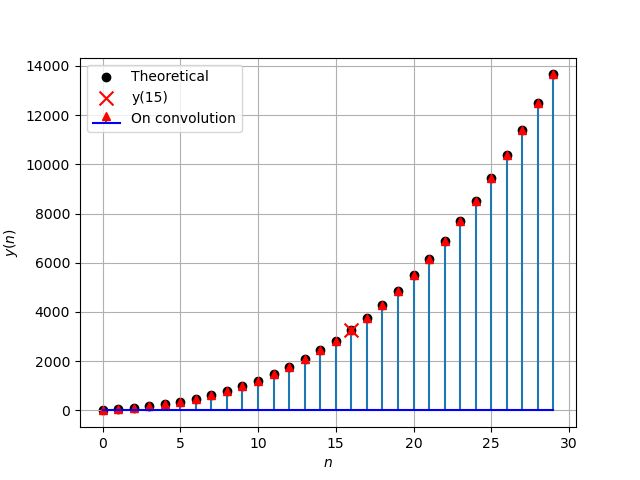
\includegraphics[width=\columnwidth]{ncert-maths/11/9/4/5/figs/plot.png}

\begin{center}
    \caption{Simulation v/s theoretical}
\end{center}
\end{figure}



\pagebreak
\item A charged particle oscillates about its mean equilibrium position with a frequency of $10^9Hz$. What is the frequency of the electromagnetic waves produced by the oscillator? \\
\solution
\input{ncert-physics/12/8/6/a1.tex}
\pagebreak
\item Given below are some functions of x and t to 
represent the displacement (transverse
or longitudinal) of an elastic wave. State which of these represents \brak i travelling
wave, \brak {ii} a stationary wave or \brak {iii} none at all: \\
\begin{enumerate}
\item $y = 2\cos \brak{3x} \sin \brak{10t}$
\item $y=2\sqrt{x-vt}$
\item $y = 3\sin \brak{5x - 0.5t} + 4\cos \brak{5x - 0.5t}$
\item $y = \cos x \sin t + \cos 2x \sin 2t$
\end{enumerate}
\solution
\input{ncert-physics/11/15/13/assignment11.tex}

\pagebreak
\item For the travelling harmonic wave
$y\brak {x, t} = 2.0 \cos 2\pi \brak{10t - 0.0080 x + 0.35}$ where $x$ and $y$ are in $cm$ and $t$ in $s$. Calculate the phase difference between oscillatory
motion of two points separated by a distance of 

\begin{enumerate} [label=(\alph*)]
    \item $4 m$
    \item $0.5 m$
    \item $\lambda/2$
    \item $3\lambda/4$
\end{enumerate}
\solution
\input{ncert-physics/11/15/10/ncert_11_15_10.tex}
\pagebreak
\item 
\begin{enumerate}
\item The peak voltage of an AC supply is 300 V. What is the rms voltage?
\item The rms value of current in an AC circuit is 10 A. What is the peak current?
\end{enumerate}
\solution
 \iffalse
\let\negmedspace\undefined
\let\negthickspace\undefined
\documentclass[journal,12pt,twocolumn]{IEEEtran}
\usepackage{amssymb}
\usepackage{cite}
\usepackage{amsmath,amssymb,amsfonts,amsthm}
\usepackage{algorithmic}
\usepackage{graphicx}
\usepackage{textcomp}
\usepackage{xcolor}
\usepackage{txfonts}
\usepackage{listings}
\usepackage{enumitem}
\usepackage{mathtools}
\usepackage{gensymb}
\usepackage{comment}
\usepackage[breaklinks=true]{hyperref}
\usepackage{tkz-euclide} 
\usepackage{listings}
\usepackage{gvv}                                        
\def\inputGnumericTable{}                                 
\usepackage[latin1]{inputenc}                                
\usepackage{color}                                            
\usepackage{array}                                            
\usepackage{longtable}                                       
\usepackage{calc}                                             
\usepackage{multirow}                                         
\usepackage{hhline}                                           
\usepackage{ifthen}                                           
\usepackage{lscape}
\usepackage{pgfplots}
\newtheorem{theorem}{Theorem}[section]
\newtheorem{problem}{Problem}
\newtheorem{proposition}{Proposition}[section]
\newtheorem{lemma}{Lemma}[section]
\newtheorem{corollary}[theorem]{Corollary}
\newtheorem{example}{Example}[section]
\newtheorem{definition}[problem]{Definition}
\newcommand{\BEQA}{\begin{eqnarray}}
\newcommand{\EEQA}{\end{eqnarray}}
\newcommand{\define}{\stackrel{\triangle}{=}}
\theoremstyle{remark}
\newtheorem{rem}{Remark}
\begin{document}

\bibliographystyle{IEEEtran}
\vspace{3cm}

\title{NCERT Discrete-11.9.4-5}
\author{EE22BTECH11004 - Allu Lohith}

\maketitle
\newpage
\bigskip


 Find the sum of n terms of this sequence:$$5^2+6^2+7^2...+20^2$$  
\solution
\fi
\begin{table}[h!]
\centering
\renewcommand{\arraystretch}{2}
\begin{tabular}{|c|p{4cm}|c|}
\hline 
\setlength{\tabcolsep}{1pt}
\textbf{Parameter}  &\textbf{Description} &\textbf{Formulae/Value} \\
\hline
n & Iteration number starting from zero till 15 & - \\
\hline
$x\brak n$ & General term of the sequence from $n=0$ to $n=15$ &$\brak{n+5}^2$  u\brak n\\
\hline
$x\brak 0$ & First term of the sequence & 5 \\
\hline
\end{tabular}

\vspace{0.5cm}
\caption{\normalsize Parameters}
\end{table}
The standard $z$ transforms,
\begin{align}
    u \brak n &\stackrel{z}{\longleftrightarrow} \frac{1}{1-z^{-1}}, \abs z >1\\
   n u\brak n &\stackrel{z}{\longleftrightarrow} \frac{z^{-1}}{\brak{1-z^{-1}}^2}, \abs z >1\\
   n^2 u\brak n &\stackrel{z}{\longleftrightarrow} \frac{z^{-1}\brak{1+z^{-1}}}{\brak{1-z^{-1}}^3}, \abs z >1
\end{align}
As 
\begin{align}
    x\brak n = \brak{n^2+10n+25}u\brak n
\end{align}
The $z$ transform of general term can be written as , 
\begin{align}
    X\brak z &= \frac{z^{-1}\brak{1+z^{-1}}}{\brak{1-z^{-1}}^3}+10\frac{z^{-1}}{\brak{1-z^{-1}}^2}+\frac{25}{1-z^{-1}} \\
    X\brak z &=  \frac{16z^{-2}-39z^{-1}+25}{\brak{1-z^{-1}}^3}; \abs{z}>1
\end{align}
On convolution for finding the sum
\begin{align}
    y\brak n= x\brak n \ast u\brak n
\end{align}
On z transform,
\begin{align}
    Y\brak z &= X \brak z \cdot U \brak z\\
    &= \brak{\frac{16z^{-2}-39z^{-1}+25}{\brak{1-z^{-1}})^3}} \cdot \frac{1}{1-z^{-1}}\\
    \implies 
    Y \brak z & = \frac{16z^{-2}-39z^{-1}+25}{\brak{1-z^{-1}}^4}; \quad \abs z >1
\end{align}
Using the contour integration to find the inverse $z$ transform,
\begin{align}
    y(n)&=\oint_c Y(z)\cdot z^{n-1}dz\\
    y(21)&=\oint_c \brak{\frac{16z^{-2}-39z^{-1}+25}{\brak{1-z^{-1}}^4}} z^{14}dz
\end{align}
As there are four poles from observation, so $m=4$
\begin{align}
    y\brak{21} &= \frac{1}{(m-1)!} \lim_{z \to a} \frac{d^{m-1}}{dz^{m-1}}\brak{(z-a)^mf(z)}\\
    &= \frac{1}{3!} \lim_{z \to 1} \frac{d^{3}}{dz^{3}}\brak{(z-1)^4 \frac{\brak{16z^{-2}-39z^{-1}+25}}{(1-z^{-1})^4} z^{14}}\\
    &= \frac{1}{6} \lim_{z \to 1} \frac{d^{3}}{dz^{3}}\brak{\brak{16z^{-2}-39z^{-1}+25}z^{18}}\\
    &= \frac{1}{6} \lim_{z \to 1} \frac{d^{3}}{dz^{3}}\brak{16z^{16}-39z^{17}+25z^{18}}\\
    &= \frac{1}{6}  \brak{16 \times 18 \times 17 \times 16+14 \times 17 \times 16 \times 15 }\\
    \implies y\brak{21}&=2840 
\end{align}
Hence the sum of the terms of the sequence is 2840.

\begin{figure}[h]
    \centering  

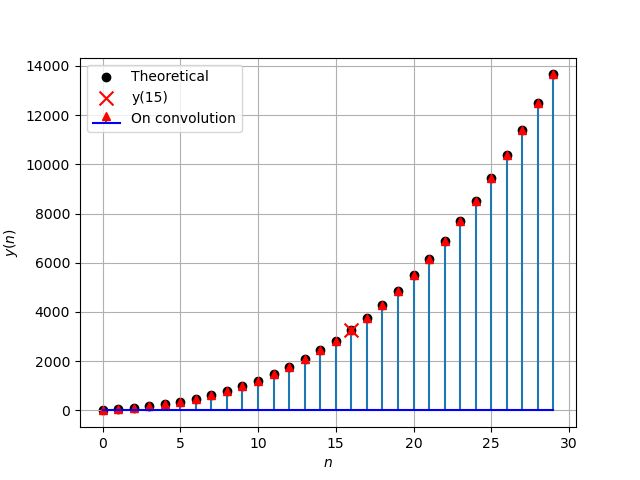
\includegraphics[width=\columnwidth]{ncert-maths/11/9/4/5/figs/plot.png}

\begin{center}
    \caption{Simulation v/s theoretical}
\end{center}
\end{figure}



\pagebreak
\item In Young’s double-slit experiment using monochromatic light of wavelength $\lambda$, the intensity of light at a point on the screen where path difference is $\lambda$, is $K$ units. What is the intensity of light at a
point where path difference is $\lambda$/3?\\

\solution

 \iffalse
\let\negmedspace\undefined
\let\negthickspace\undefined
\documentclass[journal,12pt,twocolumn]{IEEEtran}
\usepackage{amssymb}
\usepackage{cite}
\usepackage{amsmath,amssymb,amsfonts,amsthm}
\usepackage{algorithmic}
\usepackage{graphicx}
\usepackage{textcomp}
\usepackage{xcolor}
\usepackage{txfonts}
\usepackage{listings}
\usepackage{enumitem}
\usepackage{mathtools}
\usepackage{gensymb}
\usepackage{comment}
\usepackage[breaklinks=true]{hyperref}
\usepackage{tkz-euclide} 
\usepackage{listings}
\usepackage{gvv}                                        
\def\inputGnumericTable{}                                 
\usepackage[latin1]{inputenc}                                
\usepackage{color}                                            
\usepackage{array}                                            
\usepackage{longtable}                                       
\usepackage{calc}                                             
\usepackage{multirow}                                         
\usepackage{hhline}                                           
\usepackage{ifthen}                                           
\usepackage{lscape}
\usepackage{pgfplots}
\newtheorem{theorem}{Theorem}[section]
\newtheorem{problem}{Problem}
\newtheorem{proposition}{Proposition}[section]
\newtheorem{lemma}{Lemma}[section]
\newtheorem{corollary}[theorem]{Corollary}
\newtheorem{example}{Example}[section]
\newtheorem{definition}[problem]{Definition}
\newcommand{\BEQA}{\begin{eqnarray}}
\newcommand{\EEQA}{\end{eqnarray}}
\newcommand{\define}{\stackrel{\triangle}{=}}
\theoremstyle{remark}
\newtheorem{rem}{Remark}
\begin{document}

\bibliographystyle{IEEEtran}
\vspace{3cm}

\title{NCERT Discrete-11.9.4-5}
\author{EE22BTECH11004 - Allu Lohith}

\maketitle
\newpage
\bigskip


 Find the sum of n terms of this sequence:$$5^2+6^2+7^2...+20^2$$  
\solution
\fi
\begin{table}[h!]
\centering
\renewcommand{\arraystretch}{2}
\begin{tabular}{|c|p{4cm}|c|}
\hline 
\setlength{\tabcolsep}{1pt}
\textbf{Parameter}  &\textbf{Description} &\textbf{Formulae/Value} \\
\hline
n & Iteration number starting from zero till 15 & - \\
\hline
$x\brak n$ & General term of the sequence from $n=0$ to $n=15$ &$\brak{n+5}^2$  u\brak n\\
\hline
$x\brak 0$ & First term of the sequence & 5 \\
\hline
\end{tabular}

\vspace{0.5cm}
\caption{\normalsize Parameters}
\end{table}
The standard $z$ transforms,
\begin{align}
    u \brak n &\stackrel{z}{\longleftrightarrow} \frac{1}{1-z^{-1}}, \abs z >1\\
   n u\brak n &\stackrel{z}{\longleftrightarrow} \frac{z^{-1}}{\brak{1-z^{-1}}^2}, \abs z >1\\
   n^2 u\brak n &\stackrel{z}{\longleftrightarrow} \frac{z^{-1}\brak{1+z^{-1}}}{\brak{1-z^{-1}}^3}, \abs z >1
\end{align}
As 
\begin{align}
    x\brak n = \brak{n^2+10n+25}u\brak n
\end{align}
The $z$ transform of general term can be written as , 
\begin{align}
    X\brak z &= \frac{z^{-1}\brak{1+z^{-1}}}{\brak{1-z^{-1}}^3}+10\frac{z^{-1}}{\brak{1-z^{-1}}^2}+\frac{25}{1-z^{-1}} \\
    X\brak z &=  \frac{16z^{-2}-39z^{-1}+25}{\brak{1-z^{-1}}^3}; \abs{z}>1
\end{align}
On convolution for finding the sum
\begin{align}
    y\brak n= x\brak n \ast u\brak n
\end{align}
On z transform,
\begin{align}
    Y\brak z &= X \brak z \cdot U \brak z\\
    &= \brak{\frac{16z^{-2}-39z^{-1}+25}{\brak{1-z^{-1}})^3}} \cdot \frac{1}{1-z^{-1}}\\
    \implies 
    Y \brak z & = \frac{16z^{-2}-39z^{-1}+25}{\brak{1-z^{-1}}^4}; \quad \abs z >1
\end{align}
Using the contour integration to find the inverse $z$ transform,
\begin{align}
    y(n)&=\oint_c Y(z)\cdot z^{n-1}dz\\
    y(21)&=\oint_c \brak{\frac{16z^{-2}-39z^{-1}+25}{\brak{1-z^{-1}}^4}} z^{14}dz
\end{align}
As there are four poles from observation, so $m=4$
\begin{align}
    y\brak{21} &= \frac{1}{(m-1)!} \lim_{z \to a} \frac{d^{m-1}}{dz^{m-1}}\brak{(z-a)^mf(z)}\\
    &= \frac{1}{3!} \lim_{z \to 1} \frac{d^{3}}{dz^{3}}\brak{(z-1)^4 \frac{\brak{16z^{-2}-39z^{-1}+25}}{(1-z^{-1})^4} z^{14}}\\
    &= \frac{1}{6} \lim_{z \to 1} \frac{d^{3}}{dz^{3}}\brak{\brak{16z^{-2}-39z^{-1}+25}z^{18}}\\
    &= \frac{1}{6} \lim_{z \to 1} \frac{d^{3}}{dz^{3}}\brak{16z^{16}-39z^{17}+25z^{18}}\\
    &= \frac{1}{6}  \brak{16 \times 18 \times 17 \times 16+14 \times 17 \times 16 \times 15 }\\
    \implies y\brak{21}&=2840 
\end{align}
Hence the sum of the terms of the sequence is 2840.

\begin{figure}[h]
    \centering  

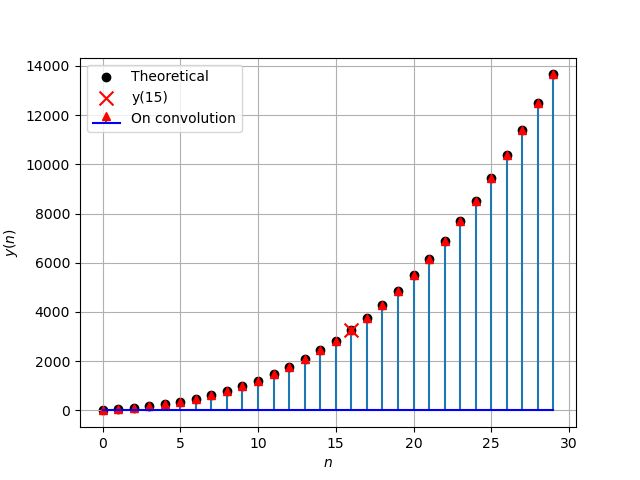
\includegraphics[width=\columnwidth]{ncert-maths/11/9/4/5/figs/plot.png}

\begin{center}
    \caption{Simulation v/s theoretical}
\end{center}
\end{figure}


\pagebreak

\item In a plane electromagnetic wave, the electric field oscillates sinusoidally at a frequency of $2.0 \text{ x } 10^{10}$ Hz and amplitude 48 $Vm^{-1}$.
\begin{enumerate}[label=(\alph*)]
    \item What is the wavelength of the wave?
    \item What is the amplitude of the oscillating magnetic field?
    \item Show that the average energy density of the $\vec{E}$ field equals the
average energy density of the $\vec{B}$ field. $[c = 3 \text{ x } 10^{8}ms^{-1} ]$
\end{enumerate}

\item \begin{enumerate}
\item For the wave on the string $y(x, t) = 0.06 \sin(\frac{2\pi x}{3}) \cos(120\pi t)$ , do all the points on the string     oscillate with the same (a)frequency , (b)phase , (c)amplitude ? Explain your answers. \\

 \item What is the amplitude of a point 0.375m away from one end? \\
 \end{enumerate}
 \solution
 \pagebreak
 
 \item 
 A transverse harmonic wave on a string is described by
\begin{align}
    y\brak{x,t}=3.0 \sin\brak{36t+0.018x+\frac{\pi}{4}}
\end{align}
where $x$ and $y$ are in cm and $t$ in s. The positive direction of $x$ is from left to right.
\begin{enumerate}[label=(\alph*)]
    \item Is this a travelling wave or a stationary wave? If it is travelling, what are the speed and direction of its propogation?
    \item What are its amplitude and frequency?
    \item What is the initial phase at the origin?
    \item  What is the least distance between two succesive crests in the wave?
\end{enumerate}

\solution
\pagebreak

\item In deriving the single slit diffraction pattern, it was stated that the intensity is zero at angles of $\frac{n\lambda}{a}$. Justify this by suitably dividing the slit to bring out the cancellation.\\
\solution
\pagebreak

\item A 60 $\mu$ F capacitor is connected to a 110 V, 60 Hz ac supply. Determine the rms value of the current in the circuit.\\
\solution
\pagebreak

\item A charged  $30\mu F$ capacitor is connected to a $27 mH$ inductor. What is the angular frequency of free oscillations of the circuit?\\
\solution
\iffalse
\documentclass[journal,12pt,twocolumn]{IEEEtran}
\usepackage{cite}
\usepackage{amsmath,amssymb,amsfonts,amsthm}
\usepackage{algorithmic}
\usepackage{graphicx}
\usepackage{textcomp}
\usepackage{xcolor}
\usepackage{txfonts}
\usepackage{listings}
\usepackage{enumitem}
\usepackage{mathtools}
\usepackage{float}
\usepackage{gensymb}
\usepackage{comment}
\usepackage[breaklinks=true]{hyperref}
\usepackage{tkz-euclide} 
\usepackage{listings}
\usepackage{gvv}                                        
\def\inputGnumericTable{}                                 
\usepackage[latin1]{inputenc}                                
\usepackage{color}                                            
\usepackage{array}                                            
\usepackage{longtable}                                       
\usepackage{calc}                                             
\usepackage{multirow}                                         
\usepackage{hhline}                                           
\usepackage{ifthen}                                           
\usepackage{lscape}
\usepackage{amsmath}
\newtheorem{theorem}{Theorem}[section]
\newtheorem{problem}{Problem}
\newtheorem{proposition}{Proposition}[section]
\newtheorem{lemma}{Lemma}[section]
\newtheorem{corollary}[theorem]{Corollary}
\newtheorem{example}{Example}[section]
\newtheorem{definition}[problem]{Definition}
\newcommand{\BEQA}{\begin{eqnarray}}
\newcommand{\EEQA}{\end{eqnarray}}
\newcommand{\define}{\stackrel{\triangle}{=}}
\theoremstyle{remark}
\newtheorem{rem}{Remark}

\usepackage{circuitikz} 

\begin{document}

\bibliographystyle{IEEEtran}
\vspace{3cm}

\title{NCERT Analog- 12.7.7}
\author{EE23BTECH11045 - Palavelli Srija$^{*}$}

\maketitle

\bigskip

\renewcommand{\thefigure}{\theenumi}
\renewcommand{\thetable}{\theenumi}

\vspace{3cm}
\textbf{Question 12.7.7:} 
 A charged $30 \mu F$ capacitor is connected to a $27 mH$ inductor. What is the angular frequency of free oscillations of the circuit?\\
\textbf{Solution: }
\fi
\begin{table}[h!]
    \centering
    
    \begin{tabular}{|c|l|c|}
        \hline
        \textbf{Symbol} & \textbf{Description} & \textbf{Value} \\
        \hline
        \(C\) & Capacitance & \(30 \mu F\) \\
        \(L\) & Inductance & \(27 mH\) \\
        \(\omega_0\) & Angular Frequency & ??\\
        \hline
    \end{tabular}

    \caption{Input Parameters}
    \label{tab:table_omega}
\end{table}
\begin{figure}[H]
    \centering
    \begin{circuitikz}
   \draw(0, 0) to [L, l=$27\,\text{mH}$] (0, -2);
   
    \draw(0, 0) -- (3, 0);
   \draw(3, 0) to [C, l=$30\,\mu\text{F}$] (3, -2) -- (0, -2);
 \draw (2, 0) -- (3, 0) node[midway, below] {-};
    \draw (2, -2) -- (3, -2) node[midway, above] {+};
    \draw (-0.5, 0) node[ below] {+};
    \draw (-0.5, -2) node[above] {-};
 \draw (-0.25, -1) node[left] {$V_L$};
    % Draw current arrow
   \draw[<-] (1, 0) -- (2, 0) node[midway, above] {$I(t)$};
   \draw (2.5, -1) node[left] {$V_C$};
\end{circuitikz}


    \caption{LC Circuit Diagram}
    \label{fig:sr33}
\end{figure}
at $t=0^-\quad V_C=-V_0,\quad I(0)=0,\quad V_L=V_0$\\

\begin{figure}[H]
    \centering
    
\begin{circuitikz}
\tikzstyle{every node}=[font=\Large]
\draw (6.75,13.5) to[L,l={ \LARGE $sL$} ] (6.75,10.75);
\draw [](6.75,13.5) to[short] (10.75,13.5);
\draw [](6.75,10.75) to[short] (10.75,10.75);
\draw (10.75,13.5) to[C,l={ \LARGE $1/sC$}] (10.75,12);
\draw (10.75,12) to[american voltage source,l={ \LARGE $V_0/s$}] (10.75,10.75);
\draw [->, >=Stealth] (8.5,13.5) -- (8.25,13.5);
\draw (8.5,13.5) -- (8.25,13.5) node[midway, above] {$I(s)$};
\end{circuitikz}


   \caption{LC Circuit Diagram in S domain}
    \label{fig:sr32}
\end{figure}
\begin{align}
sL I(s) + \frac{1}{sC} I(s) &= \frac{V_0}{s} \\
I(s) &= \frac{V_0C}{s^2LC + 1} \\
\mathcal{L}^{-1}\{I(s)\} &= I(t) \\
I(t) &= \frac{V_0C}{\sqrt{LC}} \sin\left(t\frac{1}{\sqrt{LC}}\right) \\
I(t) &= V_0\sqrt{\frac{C}{L}} \sin\left(t\frac{1}{\sqrt{LC}}\right)
\end{align}

Net impedence of LC circuit \\
\begin{align}
Z&=R_L +R_C \\
&=Ls + \dfrac{1}{sC} 
\end{align}
At resonance, the resistance of capacitor and inductor cancel out as follows:
\begin{align}
    Ls + \dfrac{1}{sC} &= 0\\
    \implies s &= j\dfrac{1}{\sqrt{LC}} \label{eq:sr20}
\end{align}
$s$ can be expressed in terms of angular resonance frequency as
\begin{equation}
    s = j\omega_0 \label{eq:sr21}
\end{equation}
on comparing \eqref{eq:sr20} and \eqref{eq:sr21}
\begin{equation}
    \omega_0 = \dfrac{1}{\sqrt{LC}}
\end{equation}
\begin{align}
\omega_0 &= \frac{1}{\sqrt{(30 \times 10^{-6}) \times (27 \times 10^{-3})}} \\
&= \frac{1}{\sqrt{8.1 \times 10^{-7}}}\\
& \approx 1.11 \times 10^{3} \, \text{rad/s}
\end{align}
Assuming $V_0=1$volt\\
\begin{figure}[h!]
    \centering
    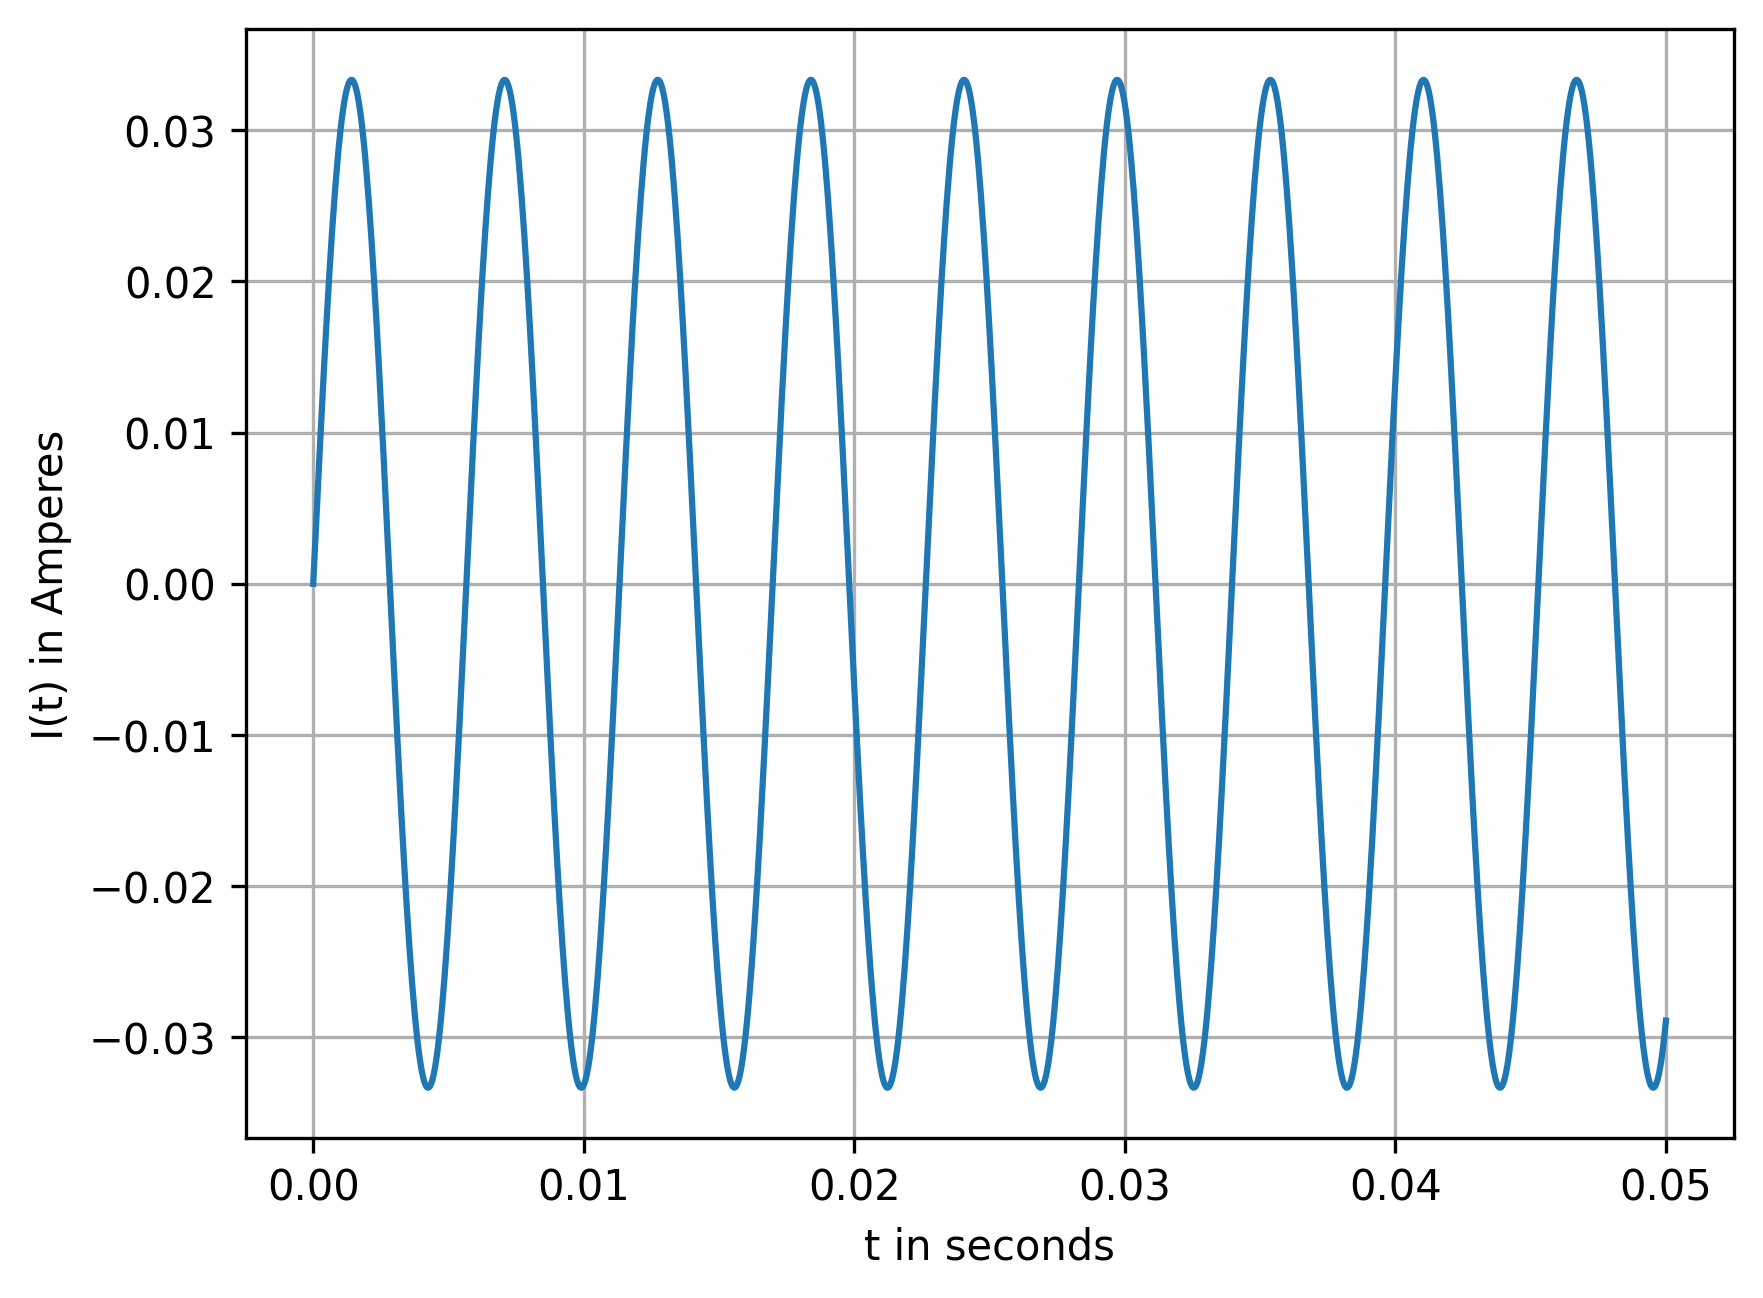
\includegraphics[width=\columnwidth,height=5cm]{ncert-physics/12/7/7/figs/p.png}
    \caption{I(t) vs t}
    \label{fig:sr31}
\end{figure}
%\end{document}


\pagebreak
\item Obtain the resonance frequency of a series LCR circuit with $L = 2.0\, H$, $C = 32\, \mu F$, and $R = 10\, \Omega$. What is the Q-value of the circuit.\\
\solution
\pagebreak
\item A charged 30 $\mu$F capacitor is connected to a 27 mH inductor. Suppose the initial charge on the capacitor is 6mC.What is the total energy stored in the circuit initially? What is the
total energy at later time? \\
\solution
\pagebreak

\item A wire stretched between two rigid supports vibrates in its fundamental mode with a frequency of $45 \, \text{Hz}$. The mass of the wire is $3.5 \times 10^{-2} \, \text{kg}$, and its linear mass density is $4.0 \times 10^{-2} \, \text{kg/m}$. The length of the wire is $0.875 \, \text{m}$. Determine the speed of a transverse wave on the string and the tension in the string.\\
\solution
\pagebreak

\item The given figure shows a series LCR circuit connected to a variable
frequency 230 V source. \\
L = 5.0 H, C = 80 $\mu$F, R = 40 $\Omega$.

\begin{figure}[h!]
\begin{center}
\begin{circuitikz}[american voltages]
      \draw (0,0)
      to[sV, l=$\varepsilon$] (0,2) 
      to[R, l=$R$, v=$V_R$] (4,2) 
      to[C, l=$C$, v=$V_C$] (4,0)
      to[L, l=$L$, v=$V_L$] (0,0);
\end{circuitikz}
\end{center}
\end{figure}

\begin{enumerate}
    \item Determine the source frequency which drives the circuit in resonance.
    \item Obtain the impedance of the circuit and the amplitude of current
at the resonating frequency.
    \item Determine the rms potential drops across the three elements of
the circuit. Show that the potential drop across the LC
combination is zero at the resonating frequency.\\
\end{enumerate}
\solution
\pagebreak

\item Q23) A narrow sound pulse (for example, a short pip by a whistle) is sent across a
	medium.\\ \brak{\text{a}} Does the pulse have a definite \brak{\text{i}} frequency, \brak{\text{ii}} wavelength, \brak{\text{iii}} speed
	of propagation?\\[1ex]\brak{\text{b}} If the pulse rate is 1 after every 20 s, (that is the whistle is
	blown for a split of second after every 20 s), Is the frequency of note produced
	by whistle equal to 1/20 or 0.05 Hz ?\\
\solution
\pagebreak
\item Suppose that the electric field part of an electromagnetic wave in vacuum given as\\ \textbf{E} =\{(3.1N/C)cos[(1.8 rad/m)y+(5.4$\times$10$^{6}$rad/s)t]\}$\vec{e_1}$ \\
(a) What is the direction of propagation ?\\
(b) What is the wavelength ? \\
(c) What is the frequency ?\\
(d) What is the amplitude of the magnetic field part of the wave?\\
(e) Write an expression for the magnetic field part of the wave.\\
\solution
\input{ncert-physics/12/8/11/analog[12.8.11].tex}
\pagebreak

\item A 44 mH inductor is connected to 220 V, 50 Hz ac supply. Determine
the rms value of the current in the circuit.\\
\solution
\input{ncert-physics/12/7/3/ac.tex}
\pagebreak

\item The 6563 \AA\, H$\alpha$ line emitted by hydrogen in a star is found to be redshifted by 15 \AA. Estimate the speed with which the star is receding from the Earth.
\solution
\pagebreak
\item The amplitude  of the magnetic part of a harmonic elctromagnetic wave is $B_0=510$nT.What is the amplitude of the electric part of the electromagnetic wave.\\
\solution
 \iffalse

\let\negmedspace\undefined
\let\negthickspace\undefined
\documentclass[journal,12pt,twocolumn]{IEEEtran}
\usepackage{cite}
\usepackage{amsmath,amssymb,amsfonts,amsthm}
\usepackage{algorithmic}
\usepackage{graphicx}
\usepackage{textcomp}
\usepackage{xcolor}
\usepackage{txfonts}
\usepackage{listings}
\usepackage{enumitem}
\usepackage{mathtools}
\usepackage{gensymb}
\usepackage{comment}
\usepackage[breaklinks=true]{hyperref}
\usepackage{tkz-euclide} 
\usepackage{listings}
\usepackage{gvv}                                        
\def\inputGnumericTable{}                                 
\usepackage[latin1]{inputenc}                                
\usepackage{color}                                            
\usepackage{array}                                            
\usepackage{longtable}                                       
\usepackage{calc}                                             
\usepackage{multirow}                                         
\usepackage{hhline}                                          
\usepackage{ifthen}                                           
\usepackage{lscape}
\usepackage{float}
\usepackage{adjustbox}

\newtheorem{theorem}{Theorem}[section]
\newtheorem{problem}{Problem}
\newtheorem{proposition}{Proposition}[section]
\newtheorem{lemma}{Lemma}[section]
\newtheorem{corollary}[theorem]{Corollary}
\newtheorem{example}{Example}[section]
\newtheorem{definition}[problem]{Definition}
\newcommand{\BEQA}{\begin{eqnarray}}
\newcommand{\EEQA}{\end{eqnarray}}
\newcommand{\define}{\stackrel{\triangle}{=}}
\theoremstyle{remark}
\parindent 0px
\newtheorem{rem}{Remark}
\begin{document}

\bibliographystyle{IEEEtran} 

\title{NCERT-12.8.7}
\author{\textbf{EE23BTECH11005} - Ambati Krishna Kaustubh% <-this % stops a space
}
\maketitle
\newpage
\bigskip

\renewcommand{\thefigure}{\arabic{figure}}
\renewcommand{\thetable}{\arabic{table}}
\section*{Question}

The amplitude  of the magnetic part of a harmonic elctromagnetic wave
is $B_0=510$nT.What is the amplitude of the electric part of the electromagnetic wave. 
   
\solution
\fi
 \begin{align}\frac{E_0}{B_0}=c\end{align}
 \begin{align}
     E_0=c*B_0
 \end{align}
 \begin{align}E_0=153V-m\end{align}
 \begin{table}[H]
    \center
    \renewcommand\thetable{1}
 

\def\arraystretch{3}
\begin{adjustbox}{width=0.5\textwidth}
    \begin{tabular}{|c|c|c|}
    \hline
        \textbf{Parameter}&\textbf{Description}&\textbf{Value}\\
        \hline
        $B_0$&Amplitude of the Electric Field&510nT\\
        \hline
        $c$&Speed of Electro Magnetic Wave&$3 \times 10^8 ms^{-1}$ \\
        \hline
        $E_0$ &amplitude of the Electric Field&153V-m \\
        \hline
       \end{tabular} 
            \end{adjustbox}
    \caption{Parameter Table}

    \label{tab:12.8.7}
\end{table}



Consider the general equation of Electric Field and Magnetic field
\begin{align}
    E=E_0\sin(\omega t-kx)
\end{align}
\begin{align}
    B=B_0\sin(\omega t-kx)
\end{align}
\begin{figure}[h]
    \centering
    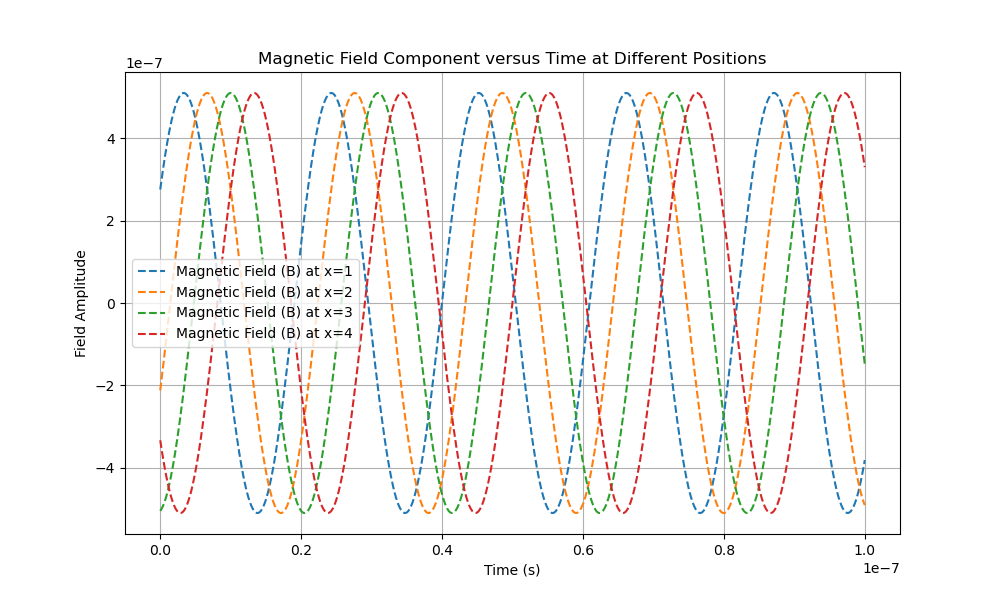
\includegraphics[width=\linewidth]{ncert-physics/12/8/7/figs/analog1.png}
    \caption{Graph of Magnetic Field vs Time}
\end{figure}
\begin{figure}[h]
    \centering
    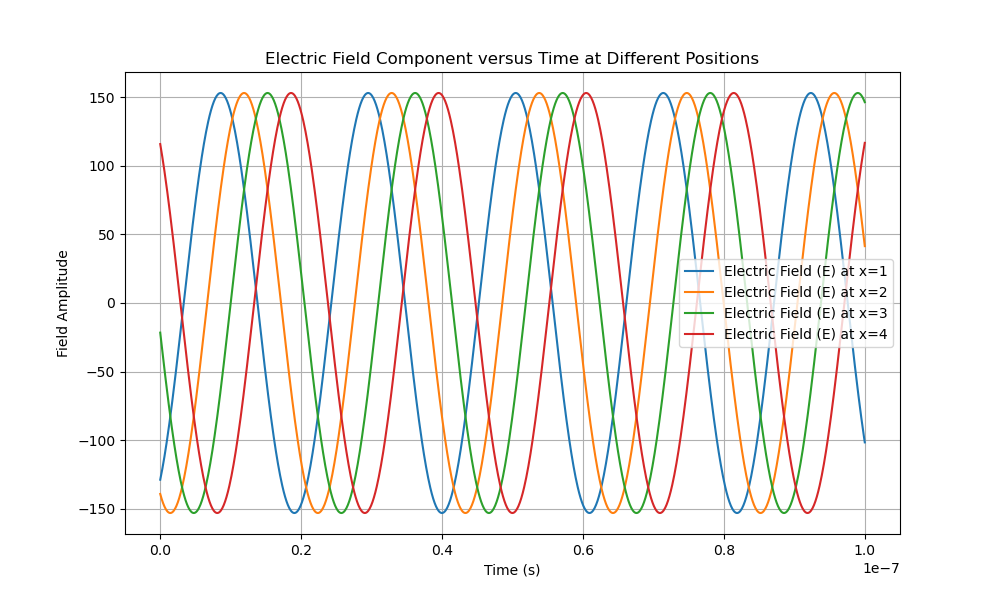
\includegraphics[width=\linewidth]{ncert-physics/12/8/7/figs/analog2.png}
    \caption{Graph of Electric Field vs Time}
\end{figure}
%\end{document}

\pagebreak

\item A 100$\mu$F capacitor in series with a 40$\Omega$ resistance is connected to a 110V, 60Hz supply.
\begin{enumerate}[label = {\brak{\alph*}}]
\item What is the maximum current in the circuit?
\item What is the time lag between the current maximum and the voltage maximum?\\
\end{enumerate}
\solution
\input{ncert-physics/12/7/15/1.2.3.tex}
\pagebreak

\item A 100 $\ohm$ resistor is connected to $220 V$, $50 Hz$ AC supply.\\
(1) What is the rms value of current in the circuit?\\
(2) What is the net power consumed over a full cycle?\\
\solution
\iffalse
\let\negmedspace\undefined
\let\negthickspace\undefined
\documentclass[journal,12pt,onecolumn]{IEEEtran}
\usepackage{cite}
\usepackage{amsmath,amssymb,amsfonts,amsthm}
\usepackage{algorithmic}
\usepackage{graphicx}
\usepackage{textcomp}
\usepackage{xcolor}
\usepackage{txfonts}
\usepackage{listings}
\usepackage{enumitem}
\usepackage{mathtools}
\usepackage{gensymb}
%\usepackage{gvv}
\usepackage{tkz-euclide} % loads  TikZ and tkz-base
\usepackage{listings}
\usetikzlibrary{positioning,arrows,shapes}


\newtheorem{theorem}{Theorem}[section]
\newtheorem{problem}{Problem}
\newtheorem{proposition}{Proposition}[section]
\newtheorem{lemma}{Lemma}[section]
\newtheorem{corollary}[theorem]{Corollary}
\newtheorem{example}{Example}[section]
\newtheorem{definition}[problem]{Definition}
%\newtheorem{thm}{Theorem}[section] 
%\newtheorem{defn}[thm]{Definition}
%\newtheorem{algorithm}{Algorithm}[section]
%\newtheorem{cor}{Corollary}
\newcommand{\BEQA}{\begin{eqnarray}}
\newcommand{\EEQA}{\end{eqnarray}}
\newcommand{\system}[1]{\stackrel{#1}{\rightarrow}}

\newcommand{\define}{\stackrel{\triangle}{=}}
\theoremstyle{remark}
\newtheorem{rem}{Remark}
%\bibliographystyle{ieeetr}
\begin{document}
%
\providecommand{\pr}[1]{\ensuremath{\Pr\left(#1\right)}}
\providecommand{\prt}[2]{\ensuremath{p_{#1}^{\left(#2\right)} }}        % own macro for this question
\providecommand{\qfunc}[1]{\ensuremath{Q\left(#1\right)}}
\providecommand{\sbrak}[1]{\ensuremath{{}\left[#1\right]}}
\providecommand{\lsbrak}[1]{\ensuremath{{}\left[#1\right.}}
\providecommand{\rsbrak}[1]{\ensuremath{{}\left.#1\right]}}
\providecommand{\brak}[1]{\ensuremath{\left(#1\right)}}
\providecommand{\lbrak}[1]{\ensuremath{\left(#1\right.}}
\providecommand{\rbrak}[1]{\ensuremath{\left.#1\right)}}
\providecommand{\cbrak}[1]{\ensuremath{\left\{#1\right\}}}
\providecommand{\lcbrak}[1]{\ensuremath{\left\{#1\right.}}
\providecommand{\rcbrak}[1]{\ensuremath{\left.#1\right\}}}
\newcommand{\sgn}{\mathop{\mathrm{sgn}}}
\providecommand{\abs}[1]{\left\vert#1\right\vert}
\providecommand{\res}[1]{\Res\displaylimits_{#1}} 
\providecommand{\norm}[1]{\left\lVert#1\right\rVert}
%\providecommand{\norm}[1]{\lVert#1\rVert}
\providecommand{\mtx}[1]{\mathbf{#1}}
\providecommand{\mean}[1]{E\left[ #1 \right]}
\providecommand{\cond}[2]{#1\middle|#2}
\providecommand{\fourier}{\overset{\mathcal{F}}{ \rightleftharpoons}}
\newenvironment{amatrix}[1]{%
  \left(\begin{array}{@{}*{#1}{c}|c@{}}
}{%
  \end{array}\right)
}
\providecommand{\hilbert}{\overset{\mathcal{H}}{ \rightleftharpoons}}
\providecommand{\system}{\overset{\mathcal{H}}{ \longleftrightarrow}}
	%\newcommand{\solution}[2]{\textbf{Solution:}{#1}}
\newcommand{\solution}{\noindent \textbf{Solution: }}
\newcommand{\cosec}{\,\text{cosec}\,}
\providecommand{\dec}[2]{\ensuremath{\overset{#1}{\underset{#2}{\gtrless}}}}
\newcommand{\myvec}[1]{\ensuremath{\begin{pmatrix}#1\end{pmatrix}}}
\newcommand{\mydet}[1]{\ensuremath{\begin{vmatrix}#1\end{vmatrix}}}
\newcommand{\myaugvec}[2]{\ensuremath{\begin{amatrix}{#1}#2\end{amatrix}}}
\providecommand{\rank}{\text{rank}}
\providecommand{\pr}[1]{\ensuremath{\Pr\left(#1\right)}}
\providecommand{\qfunc}[1]{\ensuremath{Q\left(#1\right)}}
	\newcommand*{\permcomb}[4][0mu]{{{}^{#3}\mkern#1#2_{#4}}}
\newcommand*{\perm}[1][-3mu]{\permcomb[#1]{P}}
\newcommand*{\comb}[1][-1mu]{\permcomb[#1]{C}}
\providecommand{\qfunc}[1]{\ensuremath{Q\left(#1\right)}}
\providecommand{\gauss}[2]{\mathcal{N}\ensuremath{\left(#1,#2\right)}}
\providecommand{\diff}[2]{\ensuremath{\frac{d{#1}}{d{#2}}}}
\providecommand{\myceil}[1]{\left \lceil #1 \right \rceil }
\newcommand\figref{Fig.~\ref}
\newcommand\tabref{Table~\ref}
\newcommand{\sinc}{\,\text{sinc}\,}
\newcommand{\rect}{\,\text{rect}\,}
%%
%	%\newcommand{\solution}[2]{\textbf{Solution:}{#1}}
%\newcommand{\solution}{\noindent \textbf{Solution: }}
%\newcommand{\cosec}{\,\text{cosec}\,}
%\numberwithin{equation}{section}
%\numberwithin{equation}{subsection}
%\numberwithin{problem}{section}
%\numberwithin{definition}{section}
%\makeatletter
%\@addtoreset{figure}{problem}
%\makeatother

%\let\StandardTheFigure\thefigure
\let\vec\mathbf

\bibliographystyle{IEEEtran}





\bigskip

\renewcommand{\thefigure}{\theenumi}
\renewcommand{\thetable}{\theenumi}
%\renewcommand{\theequation}{\theenumi}


\title{GATE 2023 EC}
\author{Praful Kesavadas\\ EE23BTECH11049}
\maketitle

\textbf{Q 12.7.1:}
A 100 $\ohm$ resistor is connected to $220 V$, $50 Hz$ AC supply.\\
(1) What is the rms value of current in the circuit?\\
(2) What is the net power consumed over a full cycle?

\solution\\
\fi
\begin{table}[htbp]
    \centering
    \begin{tabular}{|c|c|c|}
    \hline
   Symbol&Value&Description\\ \hline
   $V_{rms}$&220V&rms value of voltage\\ \hline
   $I_{rms}$&$\frac{V_{rms}}{R}$&rms value of current\\ \hline
   $P_{avg}$&$V_{rms} .I_{rms}$&Average power consumed per cycle\\ \hline
   $R$&100$\Omega$&Resistance \\\hline
    \end{tabular}
    
  
    \caption{Variable description} 
\end{table}\\
1)
\begin{align*}
I_{rms} &= \frac{V_{rms}}{R}\\
  &= \frac{220 V}{100 \ohm}\\
&= 2.2 A
\end{align*}
2)
\begin{align*}
\text{Net power consumed} &= \frac{V^2}{R}\\
&= \frac{220^2}{100}\\
&= 484 W
\end{align*}
\begin{figure}
\centering
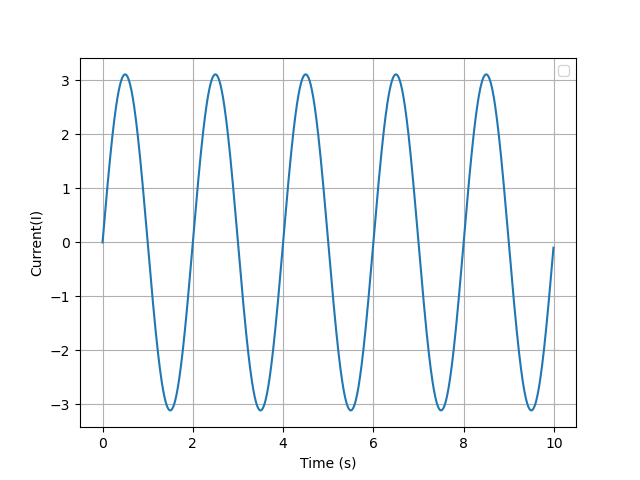
\includegraphics[width=\columnwidth]{ncert-physics/12/7/1/figs/plot1.png}
\caption{Current v/s time}
\end{figure}
%\end{document}

\pagebreak

\item  Two towers on top of two hills are $40$ km apart.This line joining them passes $50$ m above a hill halfway between the towers.What is the longest wavelength of radio waves,which can be sent between the towers without  appereciable diffraction effects?\\
\solution
\pagebreak
\item A circuit containing a 80mH inductor and a 60$\mu$F capacitor in series is connected to a 230V, 50Hz supply. The resistance of the circuit is negligible.\\
\begin{enumerate}
  \item Obtain the current amplitude and rms value.
  \item Obtain the rms value of potential drops across each element.
  \item What is the average power transferred to the inductor ?
  \item What is the average power transferred to the capacitor ?
  \item What is the total average power absorbed by the circuit ? \brak{\text{'Average' implies 'averaged over one cycle'.}}
\end{enumerate}
\solution
\pagebreak
\item A coil of inductance 0.50 H and resistance 100 $\Omega$ is connected to a 240 V, 50 Hz ac supply.\\
(a) What is the maximum current in the coil?\\		
(b) What is the time lag between the voltage maximum and the current maximum?\\
\solution
\pagebreak

\item A plane electromagnetic wave travels in vacuum along the \(z\)-direction. What can you say about the directions of its electric (\(\mathbf{E}\)) and magnetic (\(\mathbf{B}\)) field vectors? If the frequency of the wave is \(30 \, \text{MHz}\), what can you say about its wavelength?\\
\solution
\pagebreak

\item
Earthquakes generate sound waves inside the earth. Unlike a gas, the earth can experience both transverse (S) and longitudinal (P) sound waves. Typically the speed of S wave is about $4.0 km/s$, and that of P wave is $8.0 km/s$. A seismograph records P and S waves from an earthquake. The first P wave arrives $4 min$ before the first S wave. Assuming the waves travel in straight line, at what distance does the
earthquake occur ?
\solution
\pagebreak

\item
A hospital uses an ultrasonic scanner to locate tumors in a tissue. What is the wavelength of sound in the tissue in which the speed of sound is $1.7 \, \text{km/s}$? The operating frequency of the scanner is $4.2 \, \text{MHz}$.
\solution
\pagebreak

\item In double-slit experiment using light of wavelength $600 nm$, the
angular width of a fringe formed on a distant screen is $0.1\degree$. What is
the spacing between the two slits?\\
\solution
\pagebreak

\item A spring having with a spring constant 1200 N$m^{-1}$ is mounted on a horizontal
table as shown in Fig.A mass of 3 kg is attached to the free end of the
spring. The mass is then pulled sideways to a distance of 2.0 cm and released.\\
Determine (i) the frequency of oscillations, (ii) maximum acceleration of the mass,
and (iii) the maximum speed of the mass.
\begin{figure}[h!]
    \centering
    \includegraphics[width=0.5\linewidth]{ncert-physics/11/14/9/figs/analog.png}
    \caption{ }

\end{figure}
\solution
\pagebreak


\item A string of mass 2.50 kg is under a tension of 200 N. The length of the stretched string is 20.0 m. If the transverse jerk is struck at one end of the string, how long does he disturbance take to reach the other end ? 
\solution
\pagebreak

\item In a Young's double-slit experiment, the slits ar e separated by $0.28$ mm and the screen is placed $1.4 m$ away. The distance between the central bright fringe and the fourth bright fringe is measured to be $1.2 cm$. Determine the wavelength of light used in the experiment.\\
\solution
\pagebreak
\item Keeping the source frequency equal to the resonating frequency of the series $LCR$ circuit, if the three elements, $L, C$, and $R$ are arranged in parallel, show that the total current in the parallel $LCR$ circuit is minimum at this frequency. Obtain the current rms value in each branch of the circuit for the elements and source specified in Exercise 7.11 for this frequency\\
   $\varepsilon =230V$, $L=5.0H$, $C=80\mu$F, $R=40\ohm$\\
\begin{circuitikz}
    \draw (0,0) to [sV, v=$\varepsilon$] (0,3);
    \draw (2,3) to [R, l=$R$] (2,0);
    \draw (4,3) to [C, l=$C$] (4,0);
    \draw (6,3) to [L, l=$L$] (6,0);
    \draw (0,0) -- (6,0);
    \draw (0,3) -- (6,3);
\end{circuitikz}
 \solution
 \iffalse
\let\negmedspace\undefined
\let\negthickspace\undefined
\documentclass[journal,12pt,twocolumn]{IEEEtran}
\usepackage{cite}
\usepackage{amsmath,amssymb,amsfonts,amsthm}
\usepackage{algorithmic}
\usepackage{graphicx}
\usepackage{textcomp}
\usepackage{xcolor}
\usepackage[justification=centering]{caption}
\usepackage{txfonts}
\usepackage{listings}
\usepackage{enumitem}
\usepackage{mathtools}
\usepackage{gensymb}
\usepackage{comment}
\usepackage[breaklinks=true]{hyperref}
\usepackage{tkz-euclide} 
\usepackage{listings}
\usepackage{gvv}                                        
\def\inputGnumericTable{}                                 
\usepackage[latin1]{inputenc}                                
\usepackage{color}                                            
\usepackage{array}                                            
\usepackage{longtable}                                       
\usepackage{calc}                                             
\usepackage{multirow}                                         
\usepackage{hhline}                                           
\usepackage{ifthen}                                           
\usepackage{lscape}
\usepackage{circuitikz}
\newtheorem{theorem}{Theorem}[section]
\newtheorem{problem}{Problem}
\newtheorem{proposition}{Proposition}[section]
\newtheorem{lemma}{Lemma}[section]
\newtheorem{corollary}[theorem]{Corollary}
\newtheorem{example}{Example}[section]
\newtheorem{definition}[problem]{Definition}
\newcommand{\BEQA}{\begin{eqnarray}}
\newcommand{\EEQA}{\end{eqnarray}}
\newcommand{\define}{\stackrel{\triangle}{=}}
\theoremstyle{remark}
\newtheorem{rem}{Remark}
\begin{document}

\bibliographystyle{IEEEtran}
\vspace{3cm}

\title{NCERT ANALOG \\12.7.17}
\author{MANOJ KUMAR (EE23BTECH11211)}
\maketitle
\newpage

\bigskip

\renewcommand{\thefigure}{\theenumi}
\renewcommand{\thetable}{\theenumi}
\textbf{Question 17:}
Keeping the source frequency equal to the resonating frequency of the series $LCR$ circuit, if the three elements, $L, C$, and $R$ are arranged in parallel, show that the total current in the parallel $LCR$ circuit is minimum at this frequency. Obtain the current rms value in each branch of the circuit for the elements and source specified in Exercise 7.11 for this frequency\\
   $\varepsilon =230V$, $L=5.0H$, $C=80\micro$F, $R=40\ohm$\\

    \begin{circuitikz}
    \draw (0,0) to [sV, v=$\varepsilon$] (0,3);
    \draw (2,3) to [R, l=$R$] (2,0);
    \draw (4,3) to [C, l=$C$] (4,0);
    \draw (6,3) to [L, l=$L$] (6,0);
    \draw (0,0) -- (6,0);
    \draw (0,3) -- (6,3);
\end{circuitikz}

\textbf{Solution:}\\
\fi
\begin{table}[!ht]
\renewcommand\thetable{1}
   \centering
\begin{tabular}{|c|c|c|}
  \hline
  \textbf{Symbol} & \textbf{Value} & \textbf{Description}\\
  \hline
  $L$ &  $50H$ & Inductance\\
  \hline 
  $C$ &  $80 \mu F$ & Capacitance\\
  \hline
  $R$ &  $40\ohm$ & Resistance\\
  \hline
  $\varepsilon$ & $230\, V$ & Voltage source\\
  \hline
   $\omega_0$ & $\frac{1}{\sqrt{LC}}$ & Resonant Angular Frequency\\
  \hline
    $I_R$ &  $5.75A$ & Rms current value in Resistance\\
  \hline
   $I_L$ &  $0.92A$ & Rms current value in Inductor\\
  \hline
    $I_C$ &  $0.92A$ & Rms current value in Capacitor\\
  \hline
\end{tabular}
\caption{Input Parameter}
  \label{Table: 12.7.17.1}
\end{table}
\\
\text{(a)}\\

\begin{circuitikz}
    \draw (0,0) to [sV, v=$\varepsilon(s)$,] (0,3);
    \draw (2,3) to [R, l=$R$] (2,0);
    \draw (4,3) to [C, l=$\frac{1}{sC}$] (4,0);
    \draw (6,3) to [L, l=$Ls$] (6,0);
    \draw (0,0) -- (6,0);
    \draw (0,3) -- (6,3);
    \draw[->] (0, 3) node[left] {$I(s)$} -- (0.5, 3);
\end{circuitikz}

The impedance of the circuit is.
 \begin{align}
     \frac{1}{z}=\frac{1}{R}+sC+\frac{1}{Ls}\\
     I(s)=V(s)\brak{\frac{1}{R}+sC+\frac{1}{Ls}}
     \label{eq:ee.2}
 \end{align}
At resonance, the circuit becomes purely resistive\\
The admittance of capacitor and inductor cancel out as follows:
  \begin{align}
    sC + \frac{1}{Ls} &= 0\\
\implies s &= j\frac{1}{\sqrt{LC}} \label{eq:ee.4}
\end{align}
$s$ can be expressed in terms of angular resonance frequency as
\begin{equation}
    s = j\omega_0 \label{eq:ee.5}
\end{equation}
Comparing \eqref{eq:ee.4} and \eqref{eq:ee.5}, we get
\begin{equation}
    \omega_0 = \frac{1}{\sqrt{LC}}
\end{equation}
Plot of Impedance vs Angular Frequency\\
Impedance is defined as
\begin{equation}
    H(s) = \frac{V(s)}{I(s)}
\end{equation}
Using \eqref{eq:ee.5},
\begin{align}
     H(s) &=\frac{1}{\frac{1}{R} + sC + \frac{1}{Ls}}\\
     \implies H(j\omega) &=\frac{1}{\frac{1}{R} + j\omega C + \frac{1}{j\omega L}}\\
     \implies \abs{H(j\omega)} &= \frac{1}{\sqrt{\frac{1}{R^2} +\brak{\omega C - \frac{1}{\omega L}}^2}}
\end{align}
\begin{figure}[!ht]
    \centering
    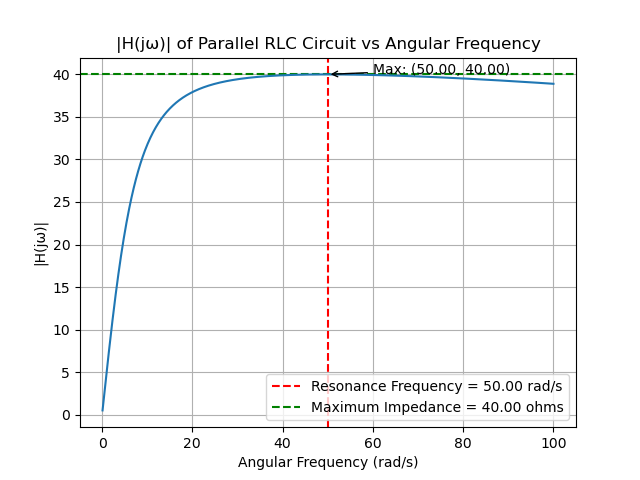
\includegraphics[width=1\linewidth]{ncert-physics/12/7/17/figs/m.png}
    \caption{Maximum impedance at resonating frequency in parallel RLC circuit}
\end{figure}

Hence it is proved that in parallel RLC circuit the total current is minimum at resonance frequency\\
   \text{(b)}\\
  At resonance frequency, Rms currents are\\
\begin{align}
\omega_0=\frac{1}{\sqrt{LC}}= 50rad/s\\
I_L=\frac{V}{\omega_0L}=\frac{230}{250}=0.92A\\
   I_C=\omega_0CV= 0.92 A\\
   I_R=\frac{V}{R}=\frac{230}{40}=5.75A
 \end{align}

 \pagebreak
\item A SONAR system fixed in a submarine operates at a frequency 40.0 kHz. An enemy submarine moves towards the SONAR with a speed of 360 km/hr. What is the frequency of sound reflected by the submarine? Take the speed of sound in water to be 1450 m/s.\\
\solution
\pagebreak

\item Figure 1.0.35 (a) shows a spring of force constant k clamped rigidly at one end and a mass $m$ attached to its free end. A force $F$ applied at the free end stretches the spring. Figure 1.0.35 (b) shows the same spring with both ends free and attached to a mass $m$ at either end. Each end of the spring in Fig. 1.0.35(b) is stretched by the same force $F$.

\begin{figure}[ht]
\caption{ }
    \includegraphics[width=0.45\textwidth]{ncert-physics/11/14/13/figs/fig1.png}
    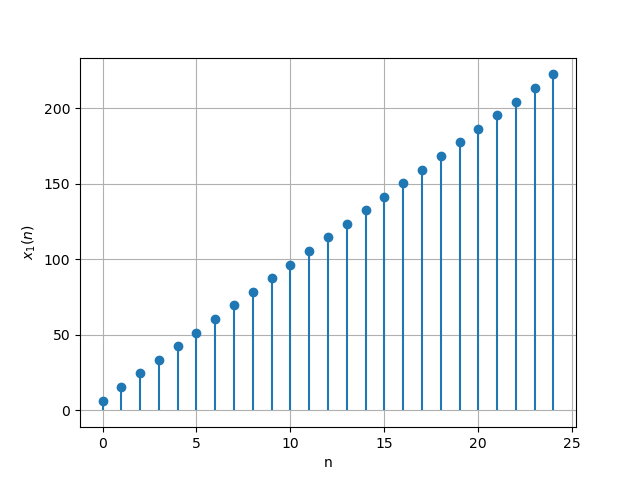
\includegraphics[width=0.45\textwidth]{ncert-physics/11/14/13/figs/fig2.png}
\end{figure}
\begin{enumerate}[label = (\alph*)]
  \item What is the maximum extension of the spring in the two cases ?    
  \item If the mass in Fig. (a) and the two masses in Fig. (b) are released, what is the
period of oscillation in each case ?
\end{enumerate}
    
\solution
\newpage

\item A bat is flitting about in a cave, navigating via ultrasonic beeps. Assume that the
sound emission frequency of the bat is 40 kHz. During one fast swoop directly
toward a flat wall surface, the bat is moving at 0.03 times the speed of sound in air.
What frequency does the bat hear reflected off the wall ? \hfill{NCERT Analog 11.15.27}\\
\solution
\pagebreak
\item One end of a long string of linear mass density $8.0 \times 10^{-3} \, \text{kg m}^{-1}$ is connected to an electrically driven tuning fork of frequency $256 \, \text{Hz}$. The other end passes over a pulley and is tied to a pan containing a mass of $90 \, \text{kg}$. The pulley end absorbs all the incoming energy so that reflected waves at this end have negligible amplitude. At $t=0$, the left end (fork end) of the string $x=0$ has zero transverse displacement ($y=0$) and is moving along positive $y$-direction. The amplitude of the wave is $5.0 \, \text{cm}$. Write down the transverse displacement $y$ as a function of $x$ and $t$ that describes the wave on the string.\hfill{NCERT Analog 11.15.24} \\
\solution
\pagebreak
\item A steel wire has a length of 12.0 m and a mass of 2.10 kg. What should be the
tension in the wire so that speed of a transverse wave on the wire equals the speed
of sound in dry air at 20 $^{\circ} C = 343ms^{-1}$ \hfill{NCERT Analog 11.15.3}\\
\solution
\pagebreak
\item What is the Brewster angle for air to glass transition?\brak{{\text{Refractive index of glass =1.5}}}\\
\solution
\pagebreak
\item A parallel beam of light with a wavelength of $500$ nm falls on a narrow slit, and the resulting diffraction pattern is observed on a screen $1$ m away. The distance to the first minimum from the center of the screen is $2.5$ mm.\\
Find the width of the slit given that $y = 0.0025$ m, $L = 1$ m, and $\lambda = 5 \times 10^{-7}$ m.\\
\solution
\pagebreak

\item Two sitar strings A and B playing the note `Ga' are slightly out of tune and produce beats of frequency $6$Hz. The tension in the string A is slightly reduced and the beat frequency is found to reduce to $3$Hz. If the original frequency of A is $324$Hz,what is the frequency of B?\\
\solution
\pagebreak

\item Which of the following functions of time represent (a) simple harmonic, (b) periodic
 but not simple harmonic, and (c) non-periodic motion? Give period for each case of periodic motion ($\omega$ is any positive constant):\\
 \begin{enumerate}
 \item $\sin\brak{\omega t}-\cos\brak{\omega t}$\\
 \item $\sin^3\brak{\omega t}$\\
 \item $3\cos\brak{\frac{\pi}{4}- 2\omega t}$\\
 \item $\cos\brak{\omega t}+\cos\brak{3\omega t}+\cos\brak{5\omega t}$\\
 \item \text{exp}\brak{-\omega^2 t^2}\\
 \item $1+\omega t+\omega^2 t^2$\\
  \end{enumerate}
 \solution
\input{ncert-physics/11/14/4/11_14_4.tex}
 \pagebreak

 \item A metre-long tube open at one end, with a movable piston at the other end, shows resonance with a fixed frequency source (a tuning fork of frequency $340$ Hz) when the tube length is $25.5$ cm or $79.3$ cm. Estimate the speed of sound in air at the temperature of the experiment. The edge effects may be neglected.\\
 \solution
 \pagebreak
\item In a double-slit experiment the angular width of a fringe is found to
be $0.2^\circ$ on a screen placed 1 m away. The wavelength of light used is
600 nm. What will be the angular width of the fringe if the entire
experimental apparatus is immersed in water? Take refractive index
of water to be $\frac{4}{3}$
\solution
\pagebreak
\item An air chamber of volume V has a neck area of cross section a into which a ball of mass m just fits and can move up down without any friction. Show that when the ball is pressed down a little and released, it executes SHM. Obtain an expression for the time period of oscillations assuming pressure-volume variations of air to be isothermal.
\solution
\pagebreak

\item
(a) The refractive index of glass is $1.5$. What is the speed of light in
glass?(Speed of light in vacuum is $3.0\times 10^{8} m s^{-1}$) \\
\\
(b) Is the speed of light in glass independent of the colour of light? If
not, which of the two colours red and violet travels slower in a
glass prism?\\
\solution
\pagebreak
\item
The motion of a particle executing simple harmonic motion is described by the
displacement function, $x(t)$ = $A$ $cos$ ($\omega$$t$ +$\phi$).
If the initial $(t = 0)$ position of the particle is $1 cm$ and its initial velocity is $\omega\quad cm/s$, what are its amplitude and initial phase angle ? The angular frequency of the particle is $\pi\quad s^{-1}$. If instead of the cosine function, we choose the sine function to describe the SHM : $x$ = $B$ $sin$ ($\omega$$t$ +$\alpha$), what are the amplitude and initial phase of the
particle with the above initial conditions.\\
\solution
\iffalse
\let\negmedspace\undefined
\let\negthickspace\undefined
\documentclass[journal,12pt,twocolumn]{IEEEtran}
\usepackage{cite}
\usepackage{amsmath,amssymb,amsfonts,amsthm}
\usepackage{algorithmic}
\usepackage{graphicx}
\usepackage{textcomp}
\usepackage{caption}
\usepackage{xcolor}
\usepackage{txfonts}
\usepackage{listings}
\usepackage{enumitem}
\usepackage{mathtools}
\usepackage{gensymb}
\usepackage[breaklinks=true]{hyperref}
\usepackage{tkz-euclide} % loads  TikZ and tkz-base
\usepackage{listings}
\usepackage{gvv}
\newtheorem{theorem}{Theorem}[section]
\newtheorem{problem}{Problem}
\newtheorem{proposition}{Proposition}[section]
\newtheorem{lemma}{Lemma}[section]
\newtheorem{corollary}[theorem]{Corollary}
\newtheorem{example}{Example}[section]
\newtheorem{definition}[problem]{Definition}
%\newtheorem{thm}{Theorem}[section] 
%\newtheorem{defn}[thm]{Definition}
%\newtheorem{algorithm}{Algorithm}[section]
%\newtheorem{cor}{Corollary}
\newcommand{\BEQA}{\begin{eqnarray}}
\newcommand{\EEQA}{\end{eqnarray}}
\newcommand{\define}{\stackrel{\triangle}{=}}
\theoremstyle{remark}
\newtheorem{rem}{Remark}

%\bibliographystyle{ieeetr}
\begin{document}
%

\bibliographystyle{IEEEtran}


\vspace{3cm}

\title{
%	\logo{
Assignment-11.14.7 

\large{EE:1205-Signals and Systems}

Indian Institute of Technology, Hyderabad
%	}
}
\author{Md Ayaan Ashraf

EE23BTECH11041
}	

\maketitle

\newpage

%\tableofcontents

\bigskip
\renewcommand{\thefigure}{\arabic{figure}}
\renewcommand{\thetable}{\arabic{table}}
%\renewcommand{\theequation}{\theenumi}
\section*{\textbf{\textit{Question}}}
The motion of a particle executing simple harmonic motion is described by the
displacement function, $x(t)$ = $A$ $cos$ ($\omega$$t$ +$\phi$).
If the initial $(t = 0)$ position of the particle is $1 cm$ and its initial velocity is $\omega\quad cm/s$, what are its amplitude and initial phase angle ? The angular frequency of the particle is $\pi\quad s^{-1}$. If instead of the cosine function, we choose the sine function to describe the SHM : $x$ = $B$ $sin$ ($\omega$$t$ +$\alpha$), what are the amplitude and initial phase of the
particle with the above initial conditions.
\section*{\textit{\textbf{Solution}}}
\fi

\begin{table}[h]
  \centering
  \begin{tabular}{|c|c|c|}
    \hline
Parameter & Description & Value \\ \hline
$x_1(0)$ & Initial position of particle in 1)& 1cm\\ \hline
$x_2(0)$ & Initial position of particle in 2)  & 1cm\\ \hline
$f$ & Frequency of particle & $\frac{\omega}{2\pi}$ \\ \hline
$x_1'(0)$ & Initial velocity of particle in 1) & $\omega$ \\ \hline
$x_2'(0)$ & Initial velocity of particle in 2)& $\omega$ \\ \hline
$\phi$ & Initial Phase Angle & ?\\
\hline
$\alpha$ & New Phase Angle & ?\\
\hline
$A$ & Initial Amplitude & ?\\
\hline
$B$ & New Amplitude & ?\\
\hline
  \end{tabular}
  \vspace{2mm}
  \caption{Parameter Table 11.14.7}
\end{table}



\begin{enumerate}
\item In \figref{Fig1_11.14.7}, the equation is
\begin{align}
   x_1(t) = A \cos(2\pi f t + \phi)  
\end{align}
Given:
\begin{align}
     x_1(0)&= A \cos(\phi) = 1 \text{ cm} \\
 x_1'(0)&= -A 2\pi f \sin(\phi) = 2\pi f \text{ cm/s} 
 \end{align}
Solving for $\phi$ and $A$:
\begin{align}
    \tan(\phi) = -1\\
\implies
\phi = -\frac{\pi}{4} \\
\implies 
A= \sqrt{2}cm
\end{align}
\begin{figure}[h]
\renewcommand\thefigure{1}
    \centering
    \includegraphics[width=0.8\columnwidth]{ncert-physics/11/14/7/figs/fig1.png}
    \caption{$x_1(t) = \sqrt{2}\cos(\pi t - \frac{\pi}{4}$)}
    \label{Fig1_11.14.7}
\end{figure}
    \item In \figref{Fig2_11.14.7}, the equation is
\begin{align}
    x_2(t) = B \sin(2\pi f t + \alpha) 
    \end{align}
    Given:\\
    \begin{align}
     x_2(0)=& B \sin(\alpha) = 1 \text{ cm} \\
    x_2'(0)=& B 2\pi f \cos(\alpha) = 2\pi f \text{ cm/s}
\end{align}
Solving for $\alpha$ and $B$:
\begin{align}
    \tan(\alpha)& = 1\\
\implies
\alpha &= \frac{\pi}{4} \\
\implies 
B &=\sqrt{2}cm
\end{align}
\begin{figure}[h]
\renewcommand\thefigure{2}
    \centering
    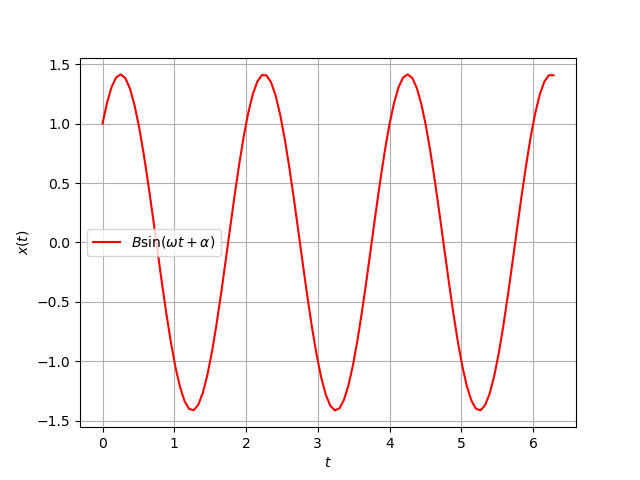
\includegraphics[width=0.8\columnwidth]{ncert-physics/11/14/7/figs/fig2.png}
    \caption{$x_2(t) = \sqrt{2}\sin(\pi t + \frac{\pi}{4})$}
    \label{Fig2_11.14.7}
\end{figure}
\end{enumerate}

\pagebreak

\item A stone dropped from the top of a tower of height $300$ m splashes into the water of a pond near the base of the tower. When is the splash heard at the top given that the speed of the sound in air is $340$ m $s^{-1}$.(g=$9.8$ m $s^{-2}$)\\
\solution
\pagebreak

\item Monochromatic light of wavelength 589nm is incident from air on a
water surface. What are the wavelength, frequency and speed of\\
(a) Reflected light?\\
(b) refracted light? Refractive index of water is 1.33.\\
\solution
\pagebreak
\item A bat emits ultrasonic sound of frequency $1000 kHz$ in air. If the sound meets a water surface, what is the wavelength of\\[0pt] \brak a the reflected sound \\[0pt]
\brak{b} the transmitted sound?\\
Speed of sound in air is $340 ms^{-1}$ and in water is $1486 ms^{-1}$.\\
\solution
\pagebreak

\item A pipe 20 cm long is closed at one end. Which harmonic mode of the pipe is

resonantly excited by a 430 Hz source ? Will the same source be in resonance with

the pipe if both ends are open? (speed of sound in air is 340 m $s^{–1}$).\\
\solution
\pagebreak

\item Figures correspond to two circular motions. The radius of the circle, the period of revolution, the initial position and the sense of revolution(i.e. clockwise or anti-clockwise) are indicated on each figure. Obtain the corresponding simple harmonic motions of the x-projections of the radius vector of resolving particle P in each case.

\begin{figure}[H]
    \centering
    \includegraphics[width=\textwidth]{ncert-physics/11/14/11/figs/qfig.pdf}
\end{figure}
\solution
\input{ncert-physics/11/14/11/1.tex}
\pagebreak

\item A steel rod $100$cm long is clamped at its middle. The fundamental frequency of the longitudinal vibrations of the rod are given to be $2.53$kHz. What is the speed of sound in steel? \\
\solution
\pagebreak

\item A train, standing in a station yard, blows a whistle of frequency $400 \, \text{Hz}$ in still air. The wind starts blowing in the direction from the yard to the station with a speed of $10 \, \text{m/s}$. What are the frequency, wavelength, and the speed of sound for an observer standing on the station's platform? Is the situation exactly identical to the case when the air is still and the observer runs towards the yard at a speed of $10\, \text{m/s}$? The speed of sound in still air can be taken as $340\, \text{m/s}$.\\
\solution
\pagebreak

\item A radio can tune in to any station in the 7.5 MHz to 12 MHz band. What is the corresponding wavelength band?\\
\solution
\pagebreak

\item A travelling harmonic wave on a string is described by $$ y(x,t) = 7.5 \sin(0.0050x + 12t + \frac{\pi}{4}) $$
\begin{enumerate}
    \item[(a)] What are the displacement and velocity of oscillation of a point at $x = 1\,\text{cm}$ and $t = 1\,\text{s}$? Is this velocity equal to the velocity of wave propagation?
    
    \item[(b)] Locate the points on the string which have the same transverse displacements and velocity as the point at $x = 1\,\text{cm}$ at $t = 2\,\text{s}$, $t = 5\,\text{s}$, and $t = 11\,\text{s}$.
\end{enumerate}
\solution
\pagebreak

\item A cylindrical piece of cork of density of base area $A$ and height h floats in a liquid of density $\rho$, The cork is depressed slightly and then released. Show that the cork oscillates up and down simple harmonically with a period $T = 2\pi\sqrt{\dfrac{h\rho}{\rho_{1}g}}$ \\
\solution
\pagebreak

\item Plot the corresponding reference circle for each of the following simple harmonic
motions. Indicate the initial (t = 0) position of the particle, the radius of the circle,and the angular speed of the rotating particle. For simplicity, the sense of rotation
may be fixed to be anticlockwise in every case: ($x$ is in cm and $t$ is in $s$)
\begin{enumerate}[label=\alph*)]
    \item $x = -2 \sin(3t + \frac{\pi}{3})$
    \item $x = \cos(\frac{\pi}{6} - t)$
    \item $x = 3 \sin(2\pi t + \frac{\pi}{4})$
    \item $x = 2 \cos(\pi t)$
\end{enumerate}

\solution
 \iffalse
\let\negmedspace\undefined
\let\negthickspace\undefined
\documentclass[journal,12pt,twocolumn]{IEEEtran}
\usepackage{amssymb}
\usepackage{cite}
\usepackage{amsmath,amssymb,amsfonts,amsthm}
\usepackage{algorithmic}
\usepackage{graphicx}
\usepackage{textcomp}
\usepackage{xcolor}
\usepackage{txfonts}
\usepackage{listings}
\usepackage{enumitem}
\usepackage{mathtools}
\usepackage{gensymb}
\usepackage{comment}
\usepackage[breaklinks=true]{hyperref}
\usepackage{tkz-euclide} 
\usepackage{listings}
\usepackage{gvv}                                        
\def\inputGnumericTable{}                                 
\usepackage[latin1]{inputenc}                                
\usepackage{color}                                            
\usepackage{array}                                            
\usepackage{longtable}                                       
\usepackage{calc}                                             
\usepackage{multirow}                                         
\usepackage{hhline}                                           
\usepackage{ifthen}                                           
\usepackage{lscape}
\usepackage{pgfplots}
\newtheorem{theorem}{Theorem}[section]
\newtheorem{problem}{Problem}
\newtheorem{proposition}{Proposition}[section]
\newtheorem{lemma}{Lemma}[section]
\newtheorem{corollary}[theorem]{Corollary}
\newtheorem{example}{Example}[section]
\newtheorem{definition}[problem]{Definition}
\newcommand{\BEQA}{\begin{eqnarray}}
\newcommand{\EEQA}{\end{eqnarray}}
\newcommand{\define}{\stackrel{\triangle}{=}}
\theoremstyle{remark}
\newtheorem{rem}{Remark}
\begin{document}

\bibliographystyle{IEEEtran}
\vspace{3cm}

\title{NCERT Discrete-11.9.4-5}
\author{EE22BTECH11004 - Allu Lohith}

\maketitle
\newpage
\bigskip


 Find the sum of n terms of this sequence:$$5^2+6^2+7^2...+20^2$$  
\solution
\fi
\begin{table}[h!]
\centering
\renewcommand{\arraystretch}{2}
\begin{tabular}{|c|p{4cm}|c|}
\hline 
\setlength{\tabcolsep}{1pt}
\textbf{Parameter}  &\textbf{Description} &\textbf{Formulae/Value} \\
\hline
n & Iteration number starting from zero till 15 & - \\
\hline
$x\brak n$ & General term of the sequence from $n=0$ to $n=15$ &$\brak{n+5}^2$  u\brak n\\
\hline
$x\brak 0$ & First term of the sequence & 5 \\
\hline
\end{tabular}

\vspace{0.5cm}
\caption{\normalsize Parameters}
\end{table}
The standard $z$ transforms,
\begin{align}
    u \brak n &\stackrel{z}{\longleftrightarrow} \frac{1}{1-z^{-1}}, \abs z >1\\
   n u\brak n &\stackrel{z}{\longleftrightarrow} \frac{z^{-1}}{\brak{1-z^{-1}}^2}, \abs z >1\\
   n^2 u\brak n &\stackrel{z}{\longleftrightarrow} \frac{z^{-1}\brak{1+z^{-1}}}{\brak{1-z^{-1}}^3}, \abs z >1
\end{align}
As 
\begin{align}
    x\brak n = \brak{n^2+10n+25}u\brak n
\end{align}
The $z$ transform of general term can be written as , 
\begin{align}
    X\brak z &= \frac{z^{-1}\brak{1+z^{-1}}}{\brak{1-z^{-1}}^3}+10\frac{z^{-1}}{\brak{1-z^{-1}}^2}+\frac{25}{1-z^{-1}} \\
    X\brak z &=  \frac{16z^{-2}-39z^{-1}+25}{\brak{1-z^{-1}}^3}; \abs{z}>1
\end{align}
On convolution for finding the sum
\begin{align}
    y\brak n= x\brak n \ast u\brak n
\end{align}
On z transform,
\begin{align}
    Y\brak z &= X \brak z \cdot U \brak z\\
    &= \brak{\frac{16z^{-2}-39z^{-1}+25}{\brak{1-z^{-1}})^3}} \cdot \frac{1}{1-z^{-1}}\\
    \implies 
    Y \brak z & = \frac{16z^{-2}-39z^{-1}+25}{\brak{1-z^{-1}}^4}; \quad \abs z >1
\end{align}
Using the contour integration to find the inverse $z$ transform,
\begin{align}
    y(n)&=\oint_c Y(z)\cdot z^{n-1}dz\\
    y(21)&=\oint_c \brak{\frac{16z^{-2}-39z^{-1}+25}{\brak{1-z^{-1}}^4}} z^{14}dz
\end{align}
As there are four poles from observation, so $m=4$
\begin{align}
    y\brak{21} &= \frac{1}{(m-1)!} \lim_{z \to a} \frac{d^{m-1}}{dz^{m-1}}\brak{(z-a)^mf(z)}\\
    &= \frac{1}{3!} \lim_{z \to 1} \frac{d^{3}}{dz^{3}}\brak{(z-1)^4 \frac{\brak{16z^{-2}-39z^{-1}+25}}{(1-z^{-1})^4} z^{14}}\\
    &= \frac{1}{6} \lim_{z \to 1} \frac{d^{3}}{dz^{3}}\brak{\brak{16z^{-2}-39z^{-1}+25}z^{18}}\\
    &= \frac{1}{6} \lim_{z \to 1} \frac{d^{3}}{dz^{3}}\brak{16z^{16}-39z^{17}+25z^{18}}\\
    &= \frac{1}{6}  \brak{16 \times 18 \times 17 \times 16+14 \times 17 \times 16 \times 15 }\\
    \implies y\brak{21}&=2840 
\end{align}
Hence the sum of the terms of the sequence is 2840.

\begin{figure}[h]
    \centering  

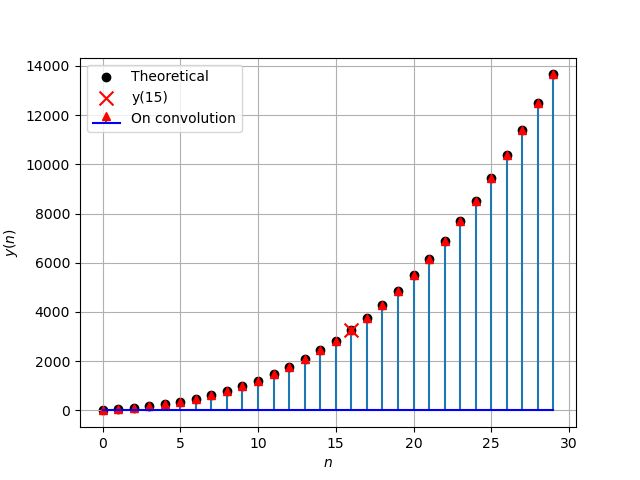
\includegraphics[width=\columnwidth]{ncert-maths/11/9/4/5/figs/plot.png}

\begin{center}
    \caption{Simulation v/s theoretical}
\end{center}
\end{figure}


\pagebreak
\end{enumerate}
